\documentclass[12pt, titlepage]{article}

\usepackage{booktabs}
\usepackage{tabularx}
\usepackage{hyperref}
\hypersetup{
    colorlinks,
    citecolor=blue,
    filecolor=black,
    linkcolor=red,
    urlcolor=blue
}
\usepackage[round]{natbib}
\usepackage{amssymb}
%% Comments

\usepackage{color}

\newif\ifcomments\commentstrue

\ifcomments
\newcommand{\authornote}[3]{\textcolor{#1}{[#3 ---#2]}}
\newcommand{\todo}[1]{\textcolor{red}{[TODO: #1]}}
\else
\newcommand{\authornote}[3]{}
\newcommand{\todo}[1]{}
\fi

\newcommand{\wss}[1]{\authornote{blue}{SS}{#1}} 
\newcommand{\plt}[1]{\authornote{magenta}{TPLT}{#1}} %For explanation of the template
\newcommand{\an}[1]{\authornote{cyan}{Author}{#1}}

%% Common Parts

\newcommand{\progname}{SPDFM} % PUT YOUR PROGRAM NAME HERE %Every program
                                % should have a name

\usepackage{graphicx}

\begin{document}

\title{Project Title: System Verification and Validation Report for \progname{}} 
\author{S. Shayan Mousavi M.}
\date{\today}
	
\maketitle

\pagenumbering{roman}

\section{Revision History}

\begin{tabularx}{\textwidth}{p{3cm}p{2cm}X}
\toprule {\bf Date} & {\bf Version} & {\bf Notes}\\
\midrule
Dec 18 2020& 1.0 & First Draft\\
\bottomrule
\end{tabularx}

\newpage

\tableofcontents

\listoftables

%\listoffigures

\newpage

\section{Symbols, Abbreviations and Acronyms}

\renewcommand{\arraystretch}{1.2}
\begin{tabular}{l l} 
  \toprule		
  \textbf{symbol} & \textbf{description}\\
  \midrule 
  T & Test\\
  VnV & verification and validation\\
  \progname{} & Surface Plasmon Dynamics Finite Method\\
  MNPBEM & Metallic NanoParticle Boundary Element Method\\
  \bottomrule
\end{tabular}\\
The complete table of symbols, abbreviations and acronyms can be found in the \href{https://github.com/shmouses/SPDFM/tree/master/docs/SRS}{SRS} document of the software. 
\newpage

\pagenumbering{arabic}

This document provides the information on validation and verification plans implemented for the \progname{} software. In this regard, the general approaches and plans are initially discussed and afterwards specific test cases and approaches for validation and verification of functional and nonfunctional requirements (can be found in \href{https://github.com/shmouses/SPDFM/tree/master/docs/SRS}{SRS}) are reviewed. VnV plans here are a combination of manual (assigned to a member of the VnV team to assess) and automated testing approaches to evaluate the correctness of the information (whether input or output) or satisfaction of a goal in \progname{}.    

\section{Implementation Validation}
\subsection{Code Walkthrough}

As is mentioned in the VnVPlan document, the checklist for code walkthrough here follows a suggested \href{http://www.mit.edu/~mbarker/ideas/review.txt}{template from MIT website}. The suggested procedure is followed by Shayan Mousavi and Alexander Pofelski. The summarized results of the session are as below:

\begin{itemize}
	\item "One list (from Handbook of Walkthroughs, Inspections, and Technical
	Reviews by Freedman and Weinberg):\\
	Function\\
	1.  Is there a concept, an underlying idea, that can be expressed
	easily in plain language?  Is it expressed in plain language in the
	implemented code?"
	
	\subitem  In general the answer is yes to this question, however, using external libraries and working with different data types can elevated level hardness in conveying the knowledge when it comes to implementation. In areas such as setting boundary conditions, and understanding impact of different types of finite elements and function spaces on the final results, still more information needs to be gathered.
	
	\item "2.  Does the function of this part have a clear place in the overall
	function of the whole, and is this function clearly expressed?
	"
	\subitem Yes, functions were clearly understood, implemented and expressed.
	
	\item"3.  Is the routine properly sheltered, so that it may perform its
	function reliably in spite of possible misuse?"
	
	\subitem The author believes so.
	
	\item "Form\\ 1.  Whatever style is adopted, is it clean and clear when taken as a
	whole?"
	
	\subitem For all the modules, form and syle is clean and clear. Moreover, PEP8 standards in coding format in python is checked using flake8 library in python for each module. All modules completely following the standard criteria.  
	
	\item "2.  Is it meaningful to all classes of readers who will see it?"
	
	\subitem Yes.
	
	\item "3.  Are there repeated code segments, whether within or between
	routines?"
	
	\subitem Not in the main modules, but this happens in the test files which are not assumed part of the module implementations in the current project.
	
	\item "4.  Are comments useful or are they simply alibis for poor coding?"
	
	\subitem Comments can be improved. 
	
	\item "5.  Is the level of detail consistent?"
	
	\subitem Yes.
	
	\item "6.  Are standard practices used?"
	
	\subitem Yes, PEP8 standard is followed.
	
	\item"7.  Is initialization properly done, and does the routine clean up
	after itself?"
	
	\subitem This area is left for the future discussion. 
	
	\item"Economy\\ 1.  Are there redundant operations for which there is no compensating
	benefit?"
	
	\subitem N/A
	
	\item "2.  Is storage use consistent, both internally and with external
	specifications?"
	
	\subitem Not discussed.
	
	\item"3.  How much will it cost to modify?  (Consider the three most likely
	future modifications.)  [my addition--and consider the three most
	likely future mistakes in modification]"
	
	\subitem N/A
	
	\item "4.  Is it simple?"
	
	\subitem The implementation of the code, yes. However, for future updates and modifications, a deep level of familiarity to the code and the modular design is required.
	
\end{itemize}



\subsection{Functional Requirements Evaluation}

\paragraph{Test R 3: Verifying light source setup}

\begin{enumerate}
	\item{\textbf{Test id1:}  Calculation of the electric field of the light source\\}
	 Test id1 is designed to compare preciseness of the external FEM solver in calculating the electric field of a plane wave in space in different frequencies and different mesh densities. In this test expected values (cosine and sinus functions) are calculated using Numpy library in python. According to the results demonstrated in Figures \ref{test1tes1-2}, \ref{test1test-3-4}, and \ref{test1test-5-6}, at low frequency (which is the frequency range that has the most applications), the difference between the expected electric field intensity and the value that FEM solver (FEniCS) interpolates, for both real and imaginary components of the field, is about $10^{-5}$ unit which is in the same order as the tolerance level and is negligible. For high frequency source the error between FEM interpolation and the expected value is in the range of $10^2$ unit but still as general sinusoidal response is still conversed simulations are acceptable, however, it should be considered that according to this test accuracy of the final result is limited by the accuracy of interpolated light source by FEM solver. 
	 As was expected, by increasing the density of mesh nodes, the error between FEM-calculated and expected values reduces. In Test id1-Test1 and Test id1-Test2, mesh geometry has 1034 nodes; this number for Test id1-Test3 and 4 is 6285, and for  Test id1-Test5 and 6 is 39827. As can be seen in Figures \ref{test1tes1-2}, \ref{test1test-3-4}, and \ref{test1test-5-6}, especially in sub-figures (f) and (h) of these figures, by increasing the number of nodes the error range window shrinks. However, increasing number of nodes increases the computational cost which can be seen in the execution time; Figure \ref{test1nodes}.
	
	 In conclusion, for the provided inputs, it is verified that \progname{} properly interpolates the light source using FEniCS toolbox, however, this interpolation is highly dependant of mesh quality (here number of nodes is targeted) and the frequency rang. For reproducing the results of this test user only needs to run \href{https://github.com/shmouses/SPDFM/tree/master/src/test_ls.py}{test\_ls.py}.  
	 
	 \begin{figure} \centering 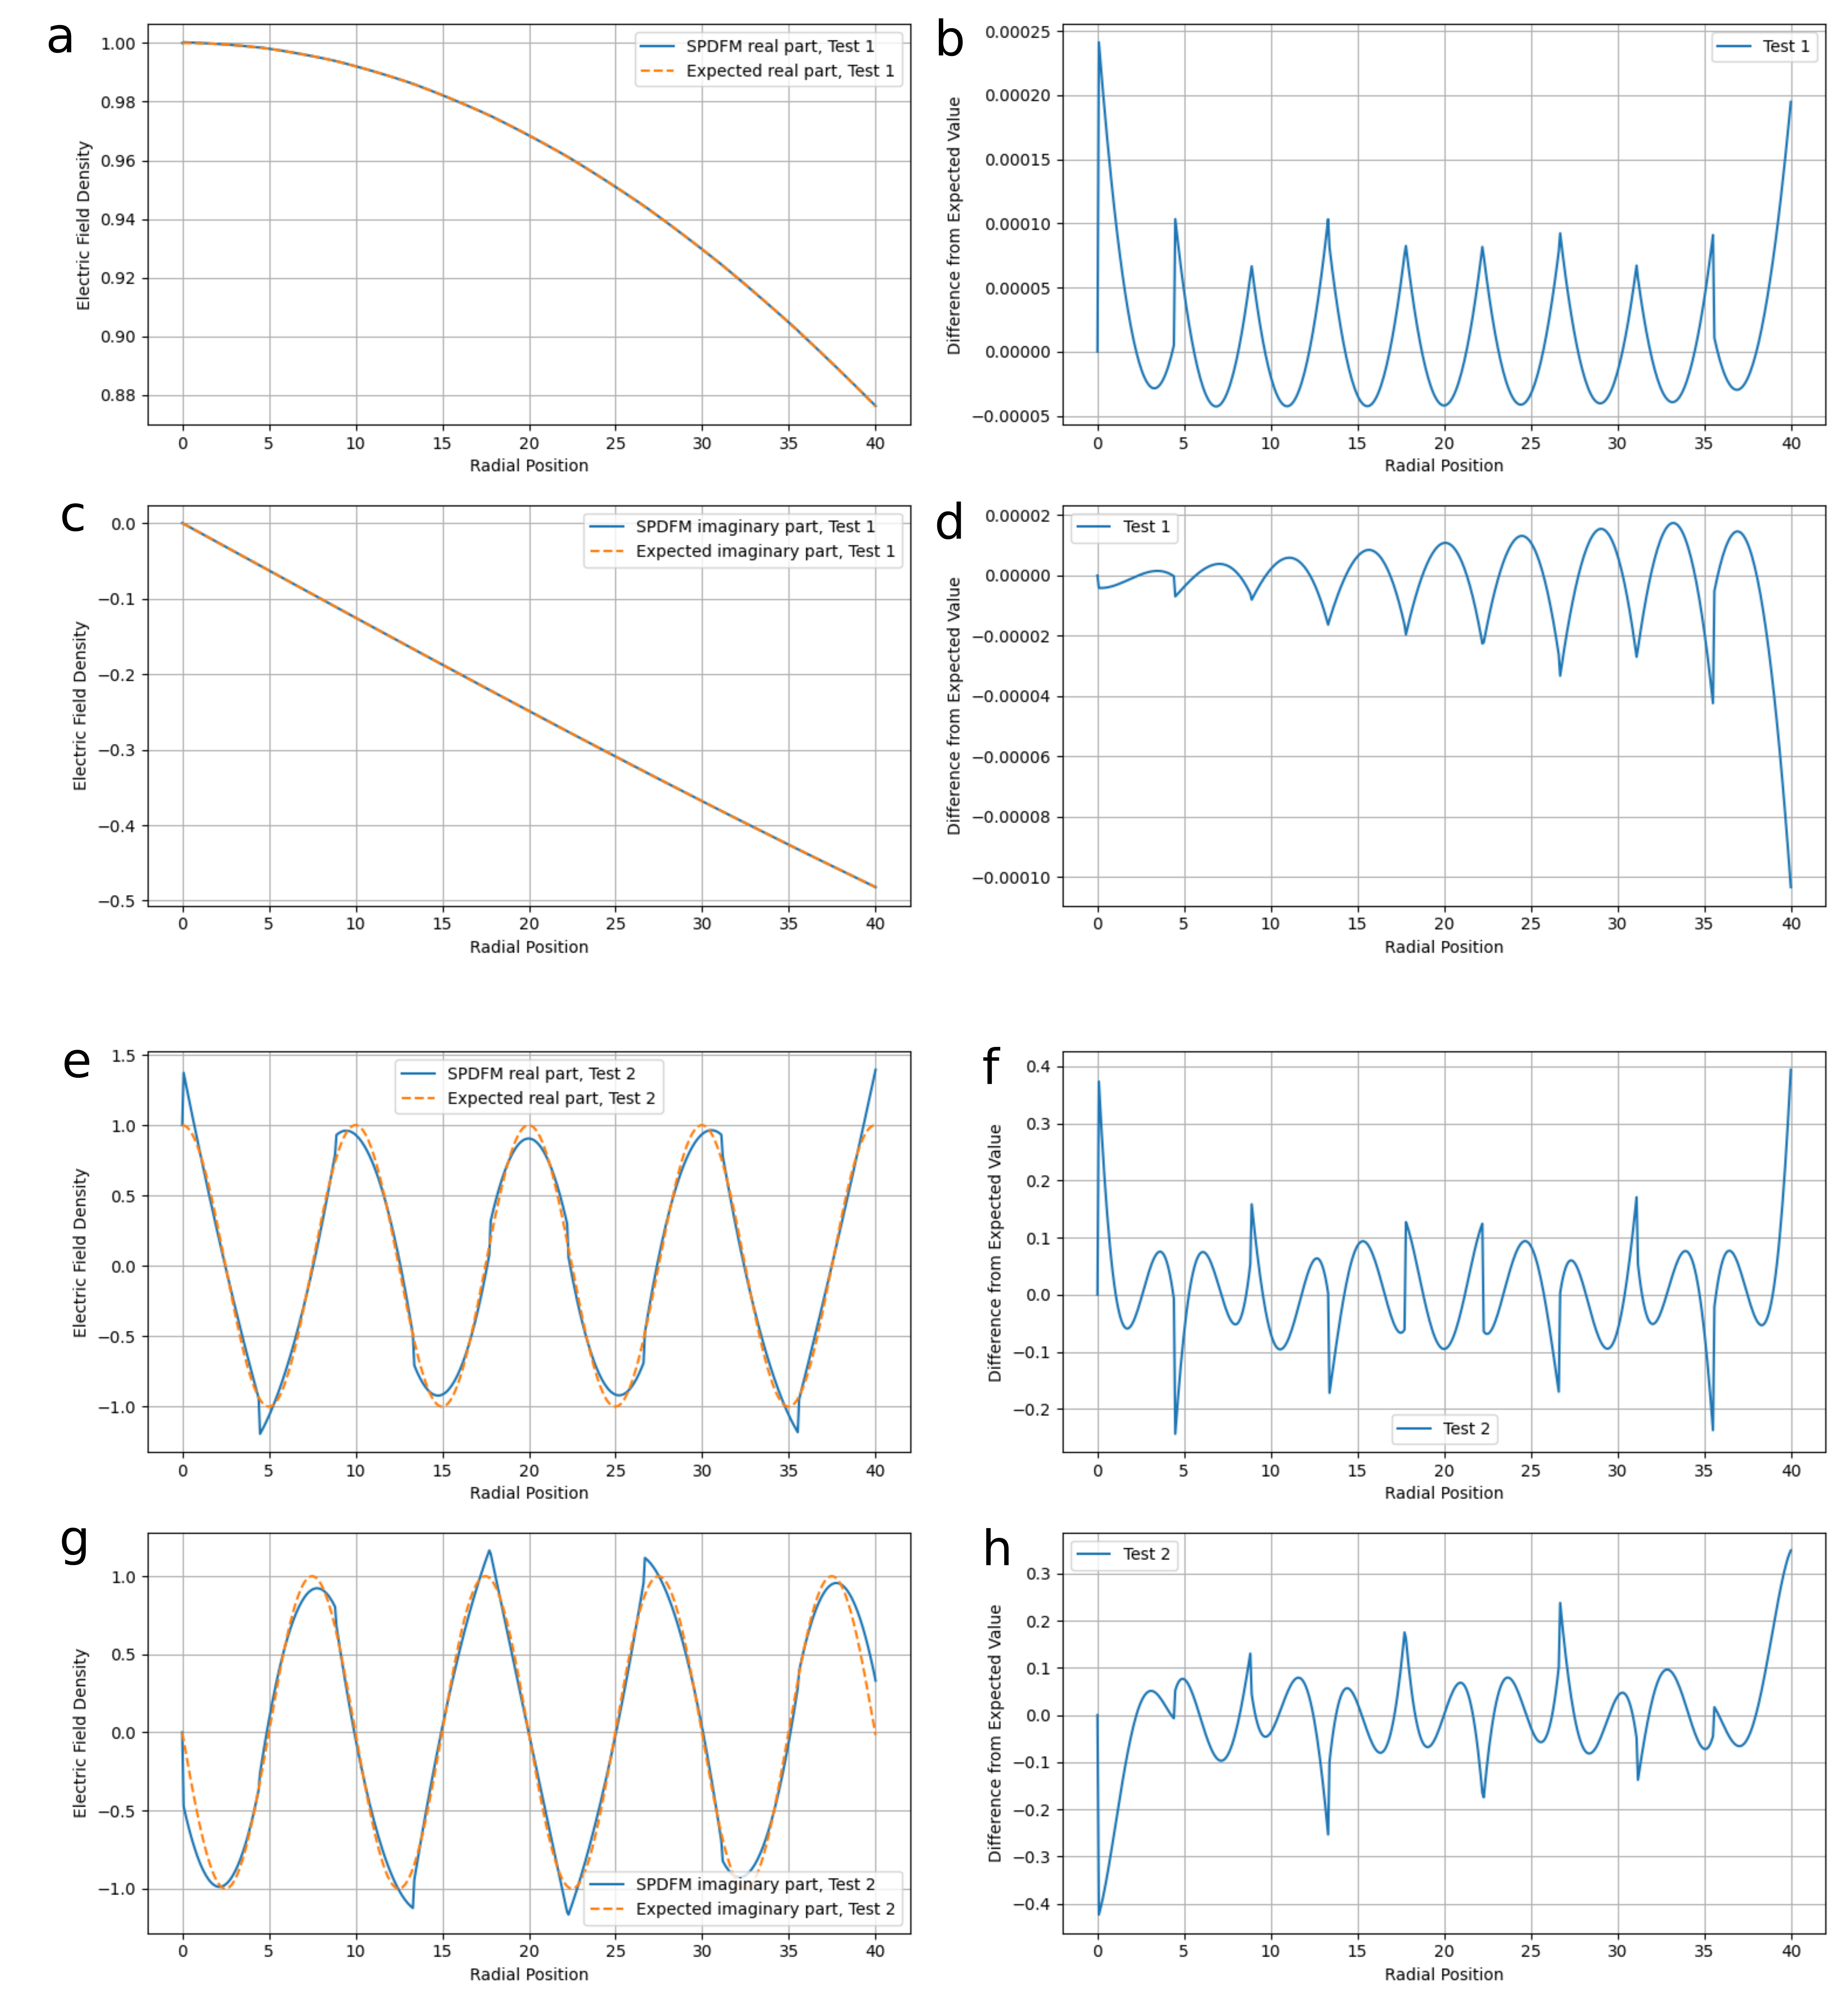
\includegraphics[width=0.7\textwidth]{R3-test1-test1-2.png} 
	 	\caption{Test id1-Test1: real component of the electric field intensity of a light source of 600 THz in a radial distance from the centre of the space calculated using \progname{} (FEM interpolation) and Numpy library in python are plotted in (a); similarly imaginary components are plotted in (c). (b) and (d) show the difference between \progname{} and Numpy calculations respectively for real component and imaginary component. Test id1-Test2: real component of the electric field intensity of a light source of 30000 THz in a radial distance from the centre of the space calculated using \progname{} (FEM interpolation) and Numpy library in python are plotted in (e); similarly imaginary components are plotted in (g). (f) and (h) show the difference between \progname{} and Numpy calculations respectively for real component and imaginary component. The meshed geometry in this test was a cube with lateral size of 40 nm and mesh consist of 1034 nodes.} \label{test1tes1-2} 
   	\end{figure}
   
    \begin{figure} \centering 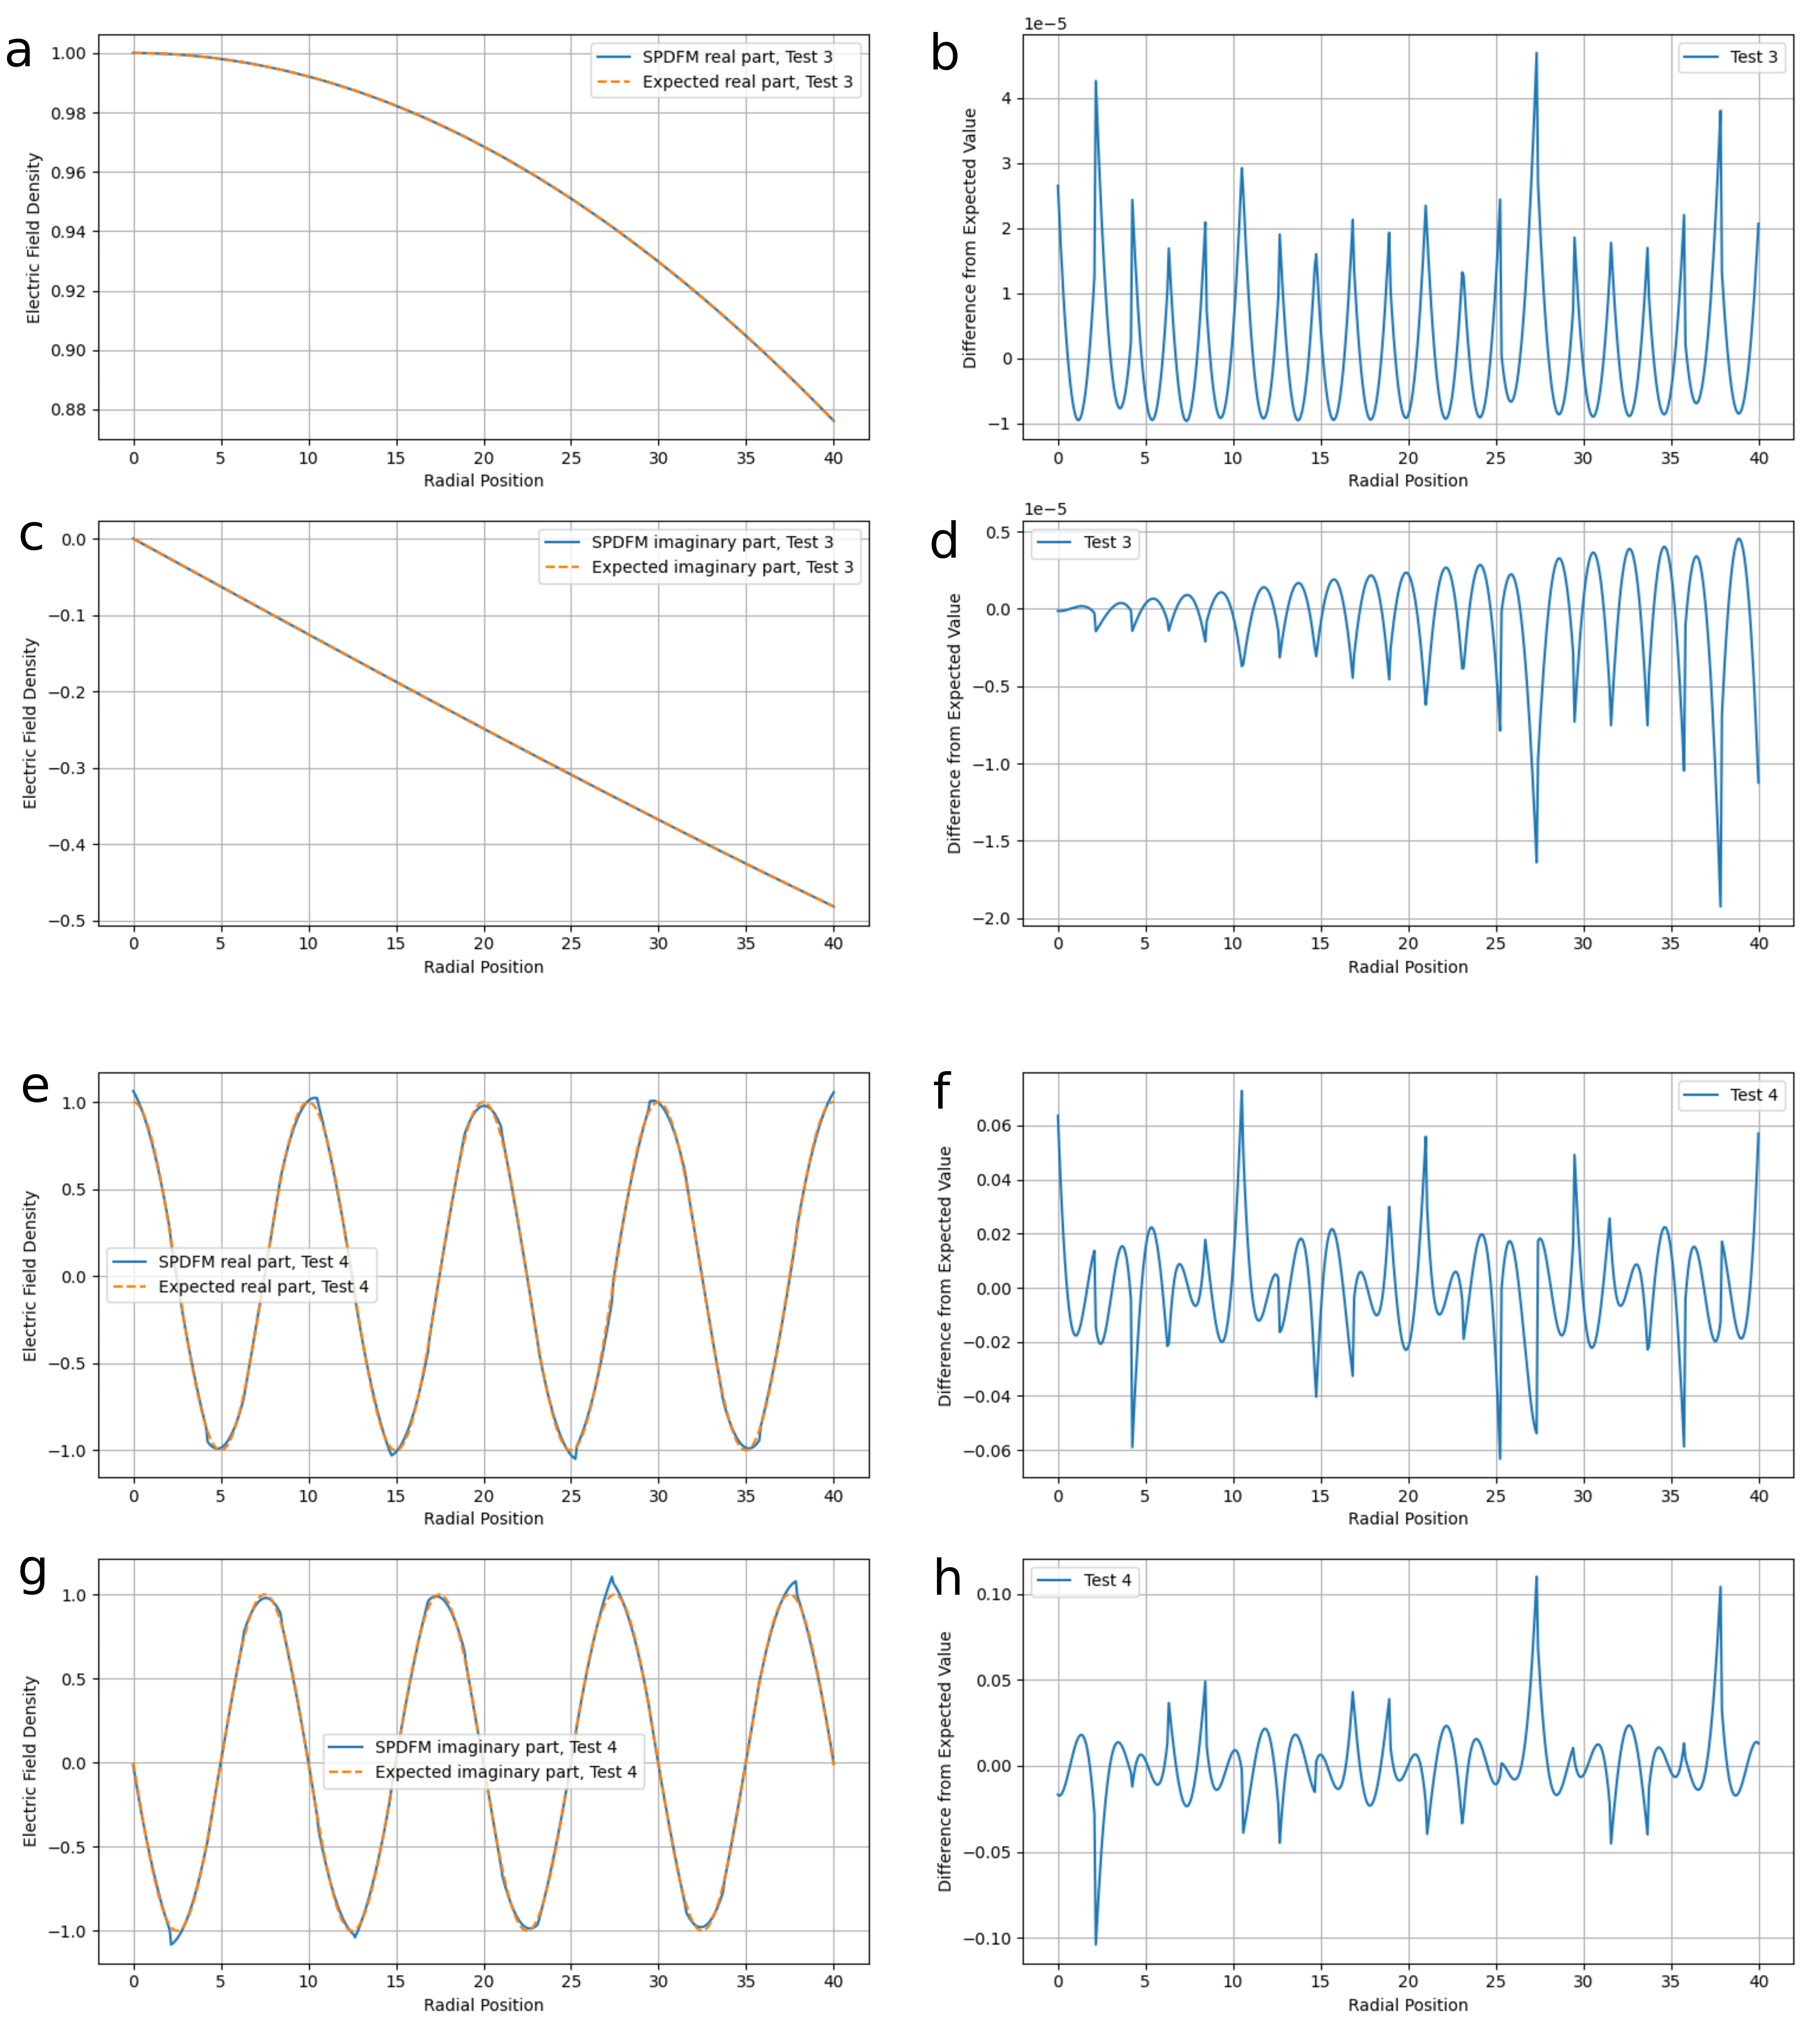
\includegraphics[width=0.7\textwidth]{R3-test1-test3-4.png}
    	\caption{Test id1-Test3: real component of the electric field intensity of a light source of 600 THz in a radial distance from the centre of the space calculated using \progname{} (FEM interpolation) and Numpy library in python are plotted in (a); similarly imaginary components are plotted in (c). (b) and (d) show the difference between \progname{} and Numpy calculations respectively for real component and imaginary component. Test id1-Test4: real component of the electric field intensity of a light source of 30000 THz in a radial distance from the centre of the space calculated using \progname{} (FEM interpolation) and Numpy library in python are plotted in (e); similarly imaginary components are plotted in (g). (f) and (h) show the difference between \progname{} and Numpy calculations respectively for real component and imaginary component. The meshed geometry in this test was a cube with lateral size of 40 nm and mesh consist of 6285 nodes.} \label{test1test-3-4}
    \end{figure}




    \begin{figure} \centering 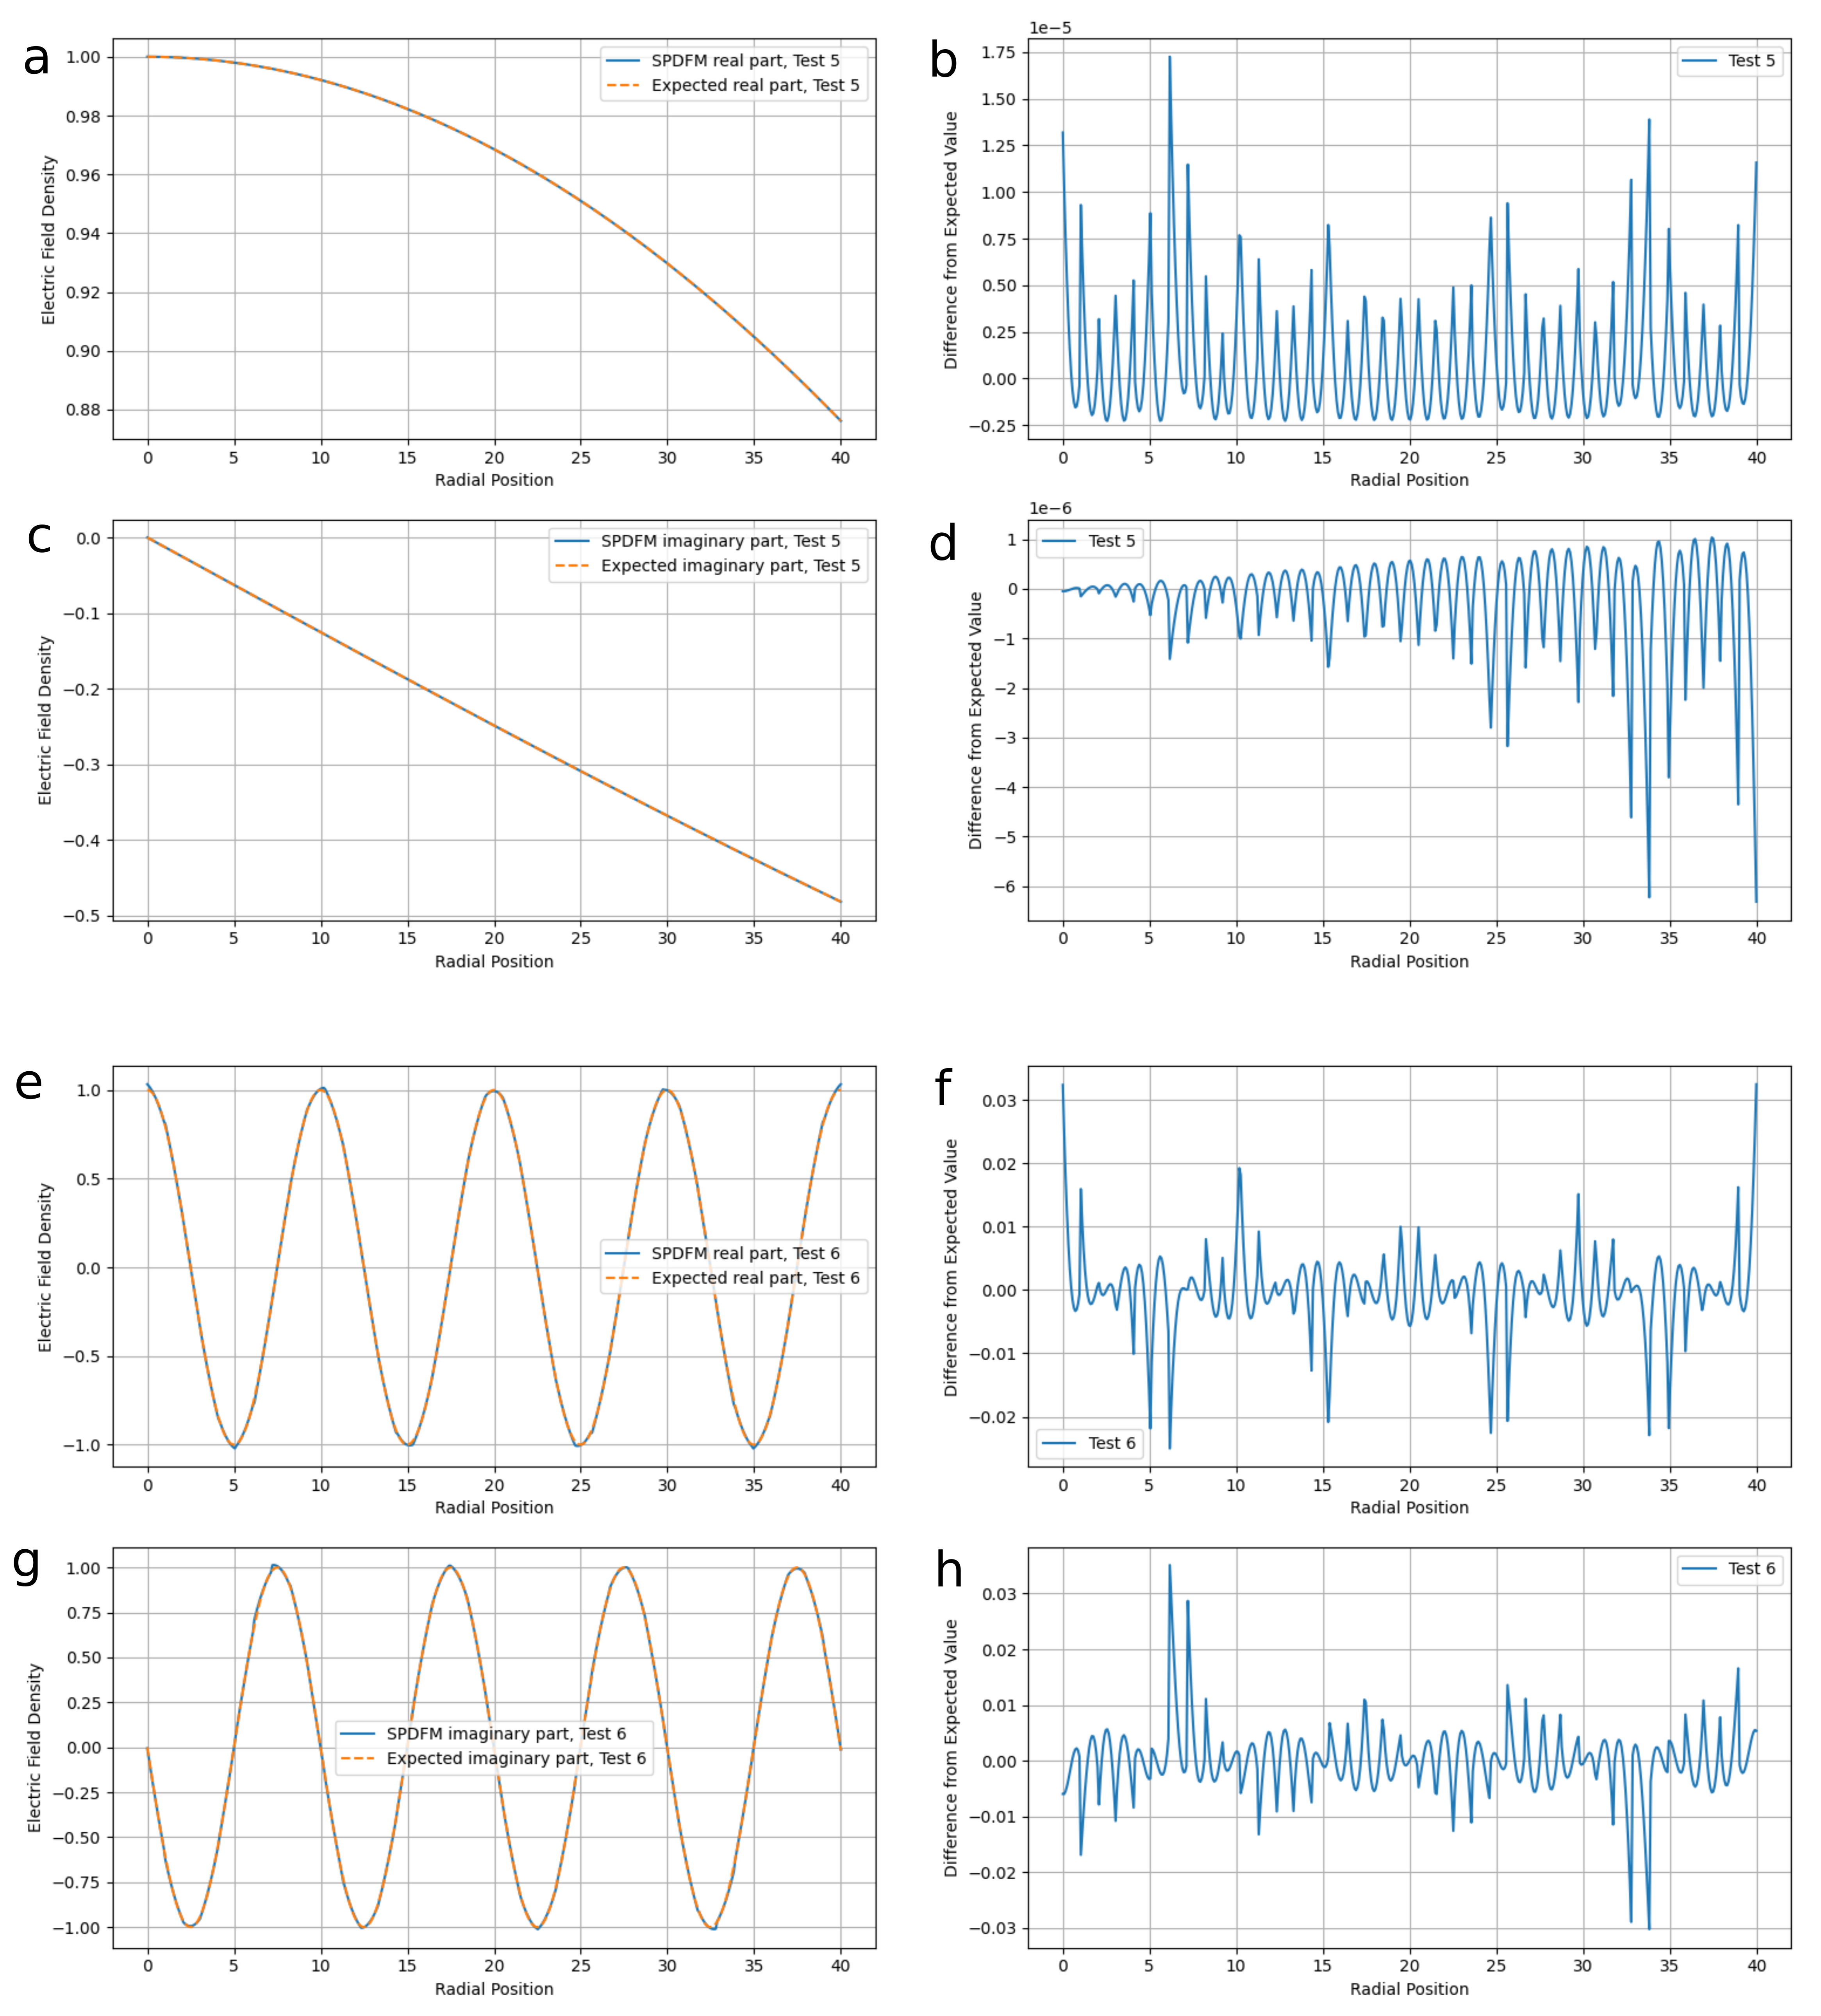
\includegraphics[width=0.7\textwidth]{R3-test1-test5-6.png}
    	\caption{Test id1-Test5: real component of the electric field intensity of a light source of 600 THz in a radial distance from the centre of the space calculated using \progname{} (FEM interpolation) and Numpy library in python are plotted in (a); similarly imaginary components are plotted in (c). (b) and (d) show the difference between \progname{} and Numpy calculations respectively for real component and imaginary component. Test id1-Test6: real component of the electric field intensity of a light source of 30000 THz in a radial distance from the centre of the space calculated using \progname{} (FEM interpolation) and Numpy library in python are plotted in (e); similarly imaginary components are plotted in (g). (f) and (h) show the difference between \progname{} and Numpy calculations respectively for real component and imaginary component. The meshed geometry in this test was a cube with lateral size of 40 nm and mesh consist of 39827 nodes.} \label{test1test-5-6} 
    \end{figure}

    \begin{figure} \centering 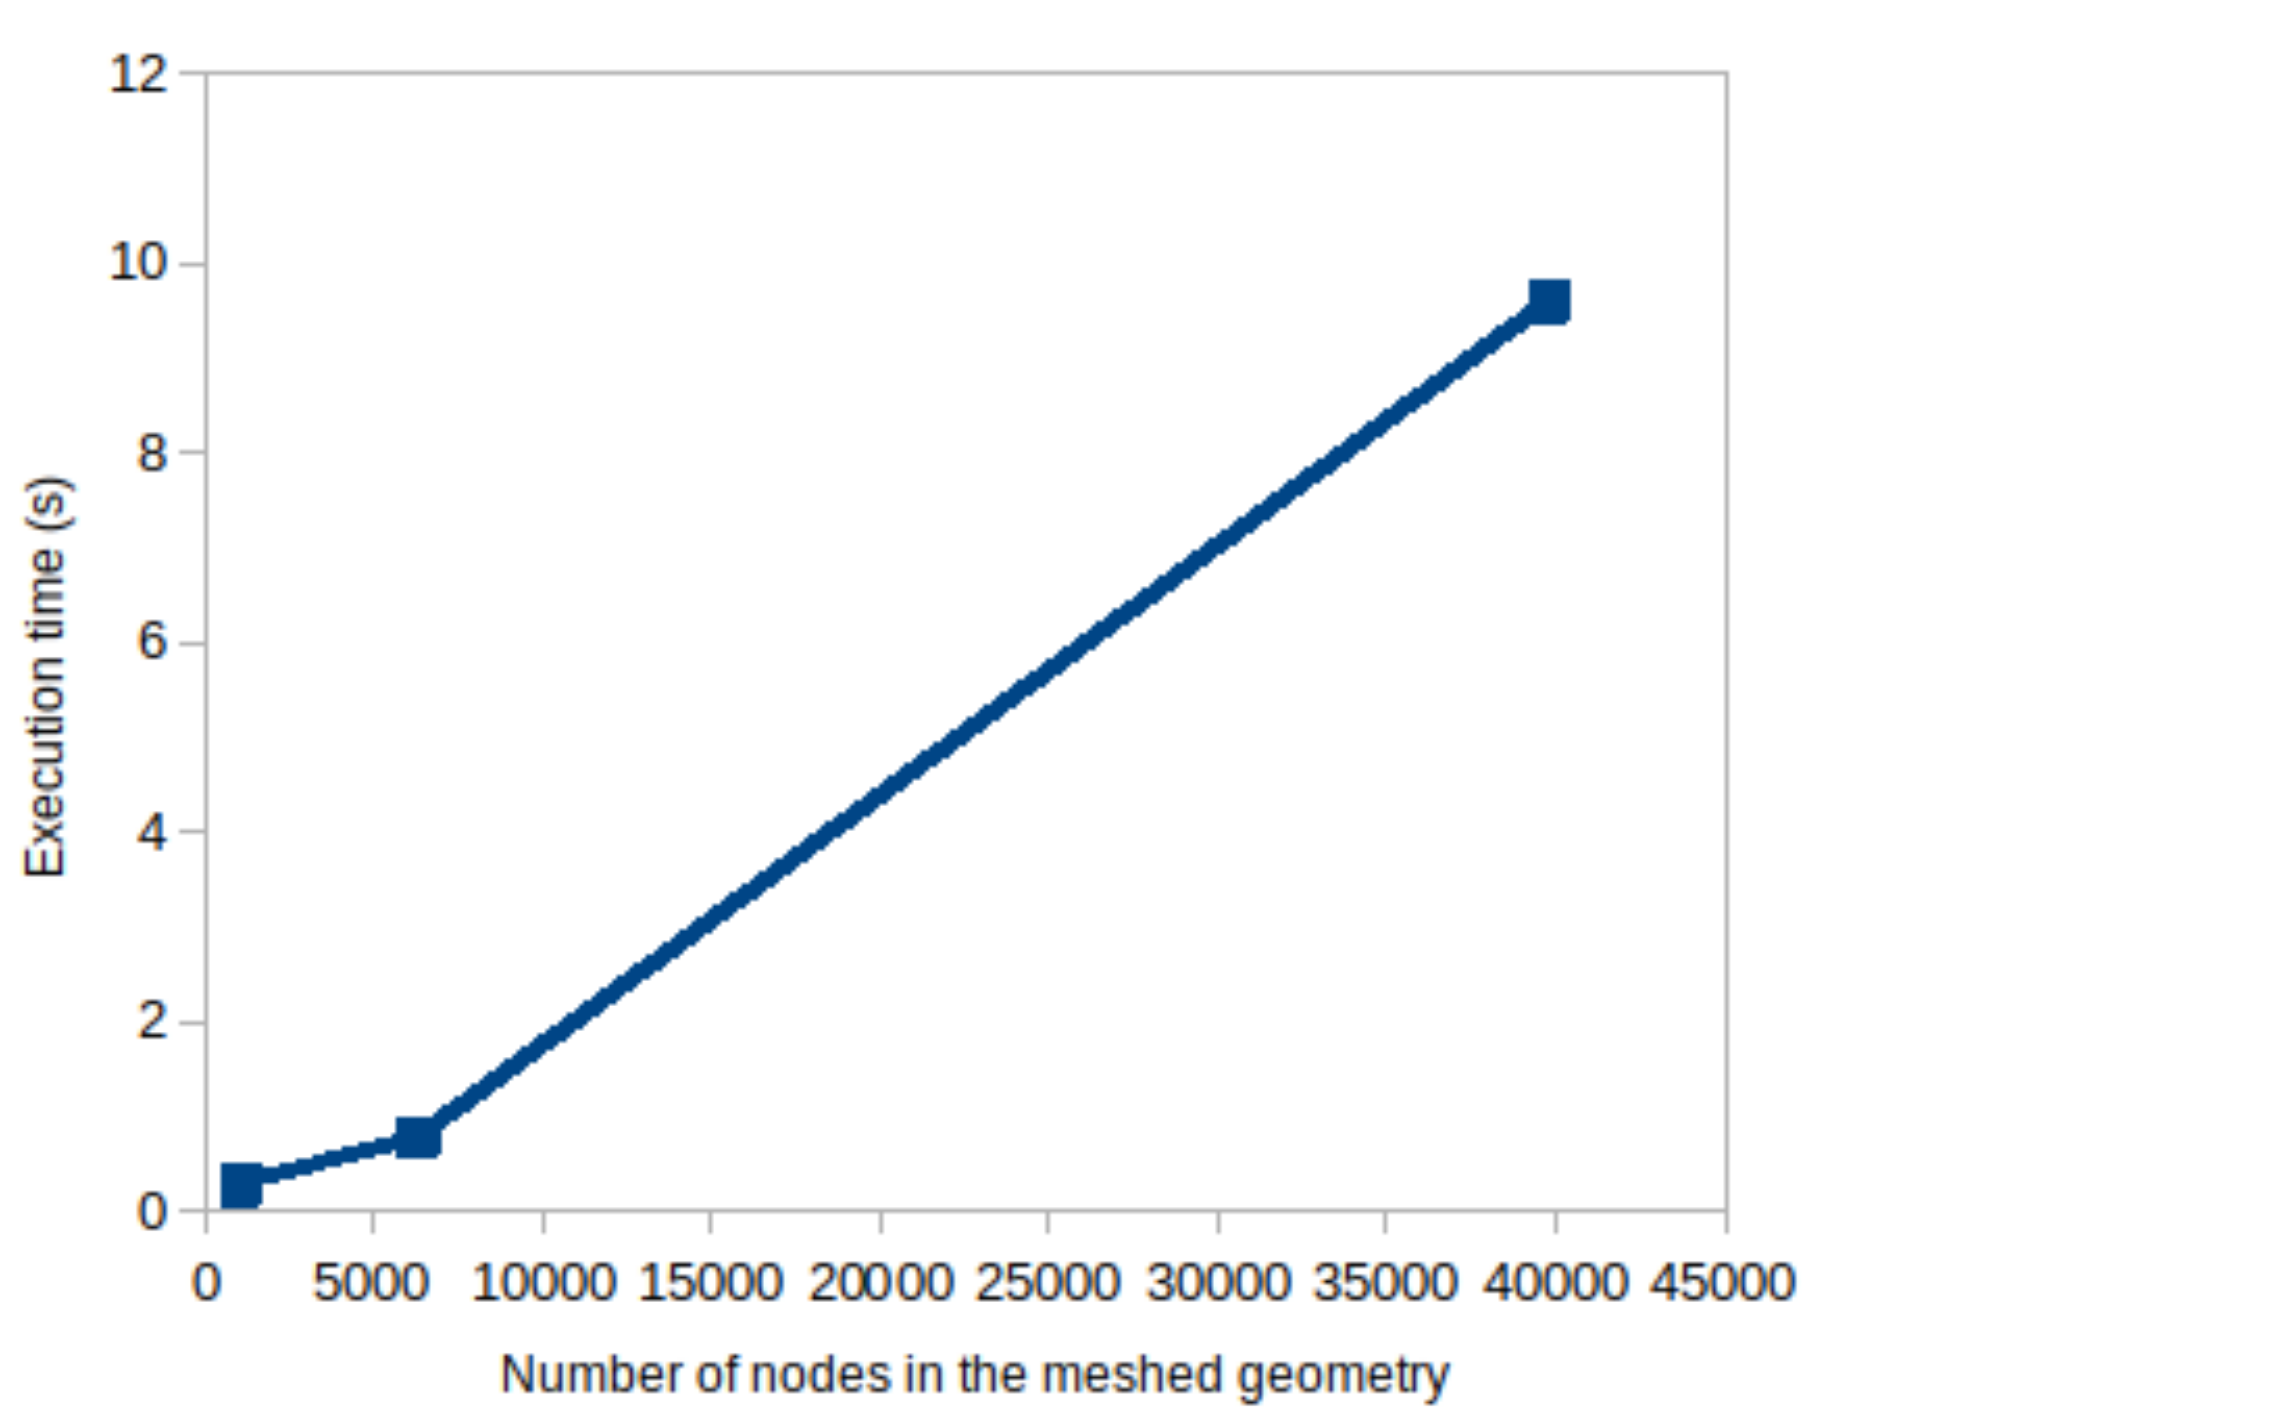
\includegraphics[width=1\textwidth]{R3-test1-nodes-time.png}
    	\caption{Test id1: Execution time for setting up the light source by \progname in meshes with different number of nodes} \label{test1nodes} 
    \end{figure}

    
\item{\textbf{Test 2:}  Visual inspection of the electric field propagation of the light source\\}


	Test 2 aims to visually inspect the distribution of interpolated electric light source calculated by \progname{} in 3D space. Although Test 1 suggests that \progname{} is capable of setting up the light source in one direction with some errors, Test 2 more concerns the general 3D distribution of the electric field in space; it is expected that reader understand that these two Tests are aiming different areas. Screen shots of visual inspection of different test cases (test cases are discussed in \href{https://github.com/shmouses/SPDFM/tree/master/docs/VnVPlan}{VnVPlan document}) are depicted in Figures \ref{R3-test2-600} and \ref{R3-test2-30000}. 3D colour map of the electric field magnitude for each input data is illustrated on the left side of the Figures \ref{R3-test2-600} and \ref{R3-test2-30000}; on the right side of the figures, magnitude of electric field at each point of the mesh that intersects with the yellow line (yellow arrow) is plotted vs. their location on the arrow (arrow is parallel to x-axis). Here real and imaginary components of test cases with of similar number of nodes and light source frequency are couple with each other (these information are engraved inside each sub-figure) and on their right side evolution of electric field with distance for both imaginary and real parts is extracted from the colour map and plotted together. 
	Figure \ref{R3-test2-600} shows spatial distribution of electric field of a 600 THz plane wave in a 40 nm cube geometry with meshes of different node density; according to this figure, the delay (phase shift) between real and imaginary part of the electric field is observed as expected and mesh density is not drastically affecting at least the visuals of the calculated field. However, this is not the case in Figure \ref{R3-test2-30000} where shows a similar parameter for 30000 THz plane wave. As can be seen in Figure \ref{R3-test2-30000}, in a mesh with less number of nodes the spatial distribution of electric field is completely disrupted and no sign of wave periodicity has remained. This shows for high frequency simulations, if mesh density is not adequate \progname{} will fail calculating the proper response (or even any response) as it fail to properly setup the light source. By increasing the node density in the mesh (top to bottom of the figure) it can be seen that the electric field distribution and oscillation becomes closer to expectations. This test shows importance of visual inspection as a complementary test to tests that are not considering all the behaviour of a function in whole space. This also shows for proper simulation of a system using \progname{}, it is crucial to first investigate behaviour of base functions in meshes of different density (this highly depends on the parameters that user inputs and should be tested in each project separately and is beyond scope of this document).      
	The pvd maps used in for conducting the visual inspection can be obtained by executing \href{https://github.com/shmouses/SPDFM/tree/master/src/test_visual_ls.py}{test\_visual\_ls.py}. The visual inspection is done in the \href{www.paraview.org}{ParaView} software.
	
	\begin{figure} \centering \includegraphics[width=0.7\textwidth]{R3-test2-600.png}
		\caption{Electric field distribution (both real and imaginary components) of the plane wave with 600 THz in a 40 nm cubic space. Test id of each test (can be matched with the information in VnVPlan document), in addition to the number of nodes in the mesh and the frequency of the light source is shown on the top-left of each colour map. Evolution of the real and imaginary electric field along yellow arrow is plotted on the right side of corresponding colour maps.} \label{R3-test2-600}  
	\end{figure}
	
	\begin{figure} \centering \includegraphics[width=0.7\textwidth]{R3-test2-30000.png}
		\caption{Test id1-Test1: real component of the electric field intensity of a light source of 600 THz in a radial distance from the centre of the space calculated using \progname{} (FEM interpolation) and Numpy library in python are plotted in (a); similarly imaginary components are plotted in (c). (b) and (d) show the difference between \progname{} and Numpy calculations respectively for real component and imaginary component. Test id1-Test2: real component of the electric field intensity of a light source of 30000 THz in a radial distance from the centre of the space calculated using \progname{} (FEM interpolation) and Numpy library in python are plotted in (e); similarly imaginary components are plotted in (g). (f) and (h) show the difference between \progname{} and Numpy calculations respectively for real component and imaginary component. The meshed geometry in this test was a cube with lateral size of 40 nm and mesh consist of 1034 nodes} \label{R3-test2-30000} 
	\end{figure}	

	
\end{enumerate}

\paragraph{Test R 4: Verifying calculated electric field and electric current density}

\begin{enumerate}
	
	\item{\textbf{Test id3:} Plasmon enhanced electric field calculation compared to boundary element simulation\\}
	
	As is explained in the VnV plan document, this test compares the simulation results obtained from \progname{} to simulation results obtained from a peer reviewed and verified boundary element method (BEM) toolbox in MATLAB, MNPBEM. 
	This test is divided to three sets of meshes with low (Set1), medium (Set2), and high density (Set3) mesh density; these comparisons are just between the three meshes in this test and when it is said a mesh has high mesh density it doesn't mean that the mesh is of high quality.
	To compare the \progname{} result with the BEM simulations, in each set there exists a particle that has only meshed on the the surface and a thoroughly meshed particle; this way impact of volume meshing and only applying the mesh on the surface was intended to be studied.  
	The expected response that is  MNPBEM simulation suggests can be found in Figure \ref{mnpbem}.
	
	 
	\begin{figure} \centering 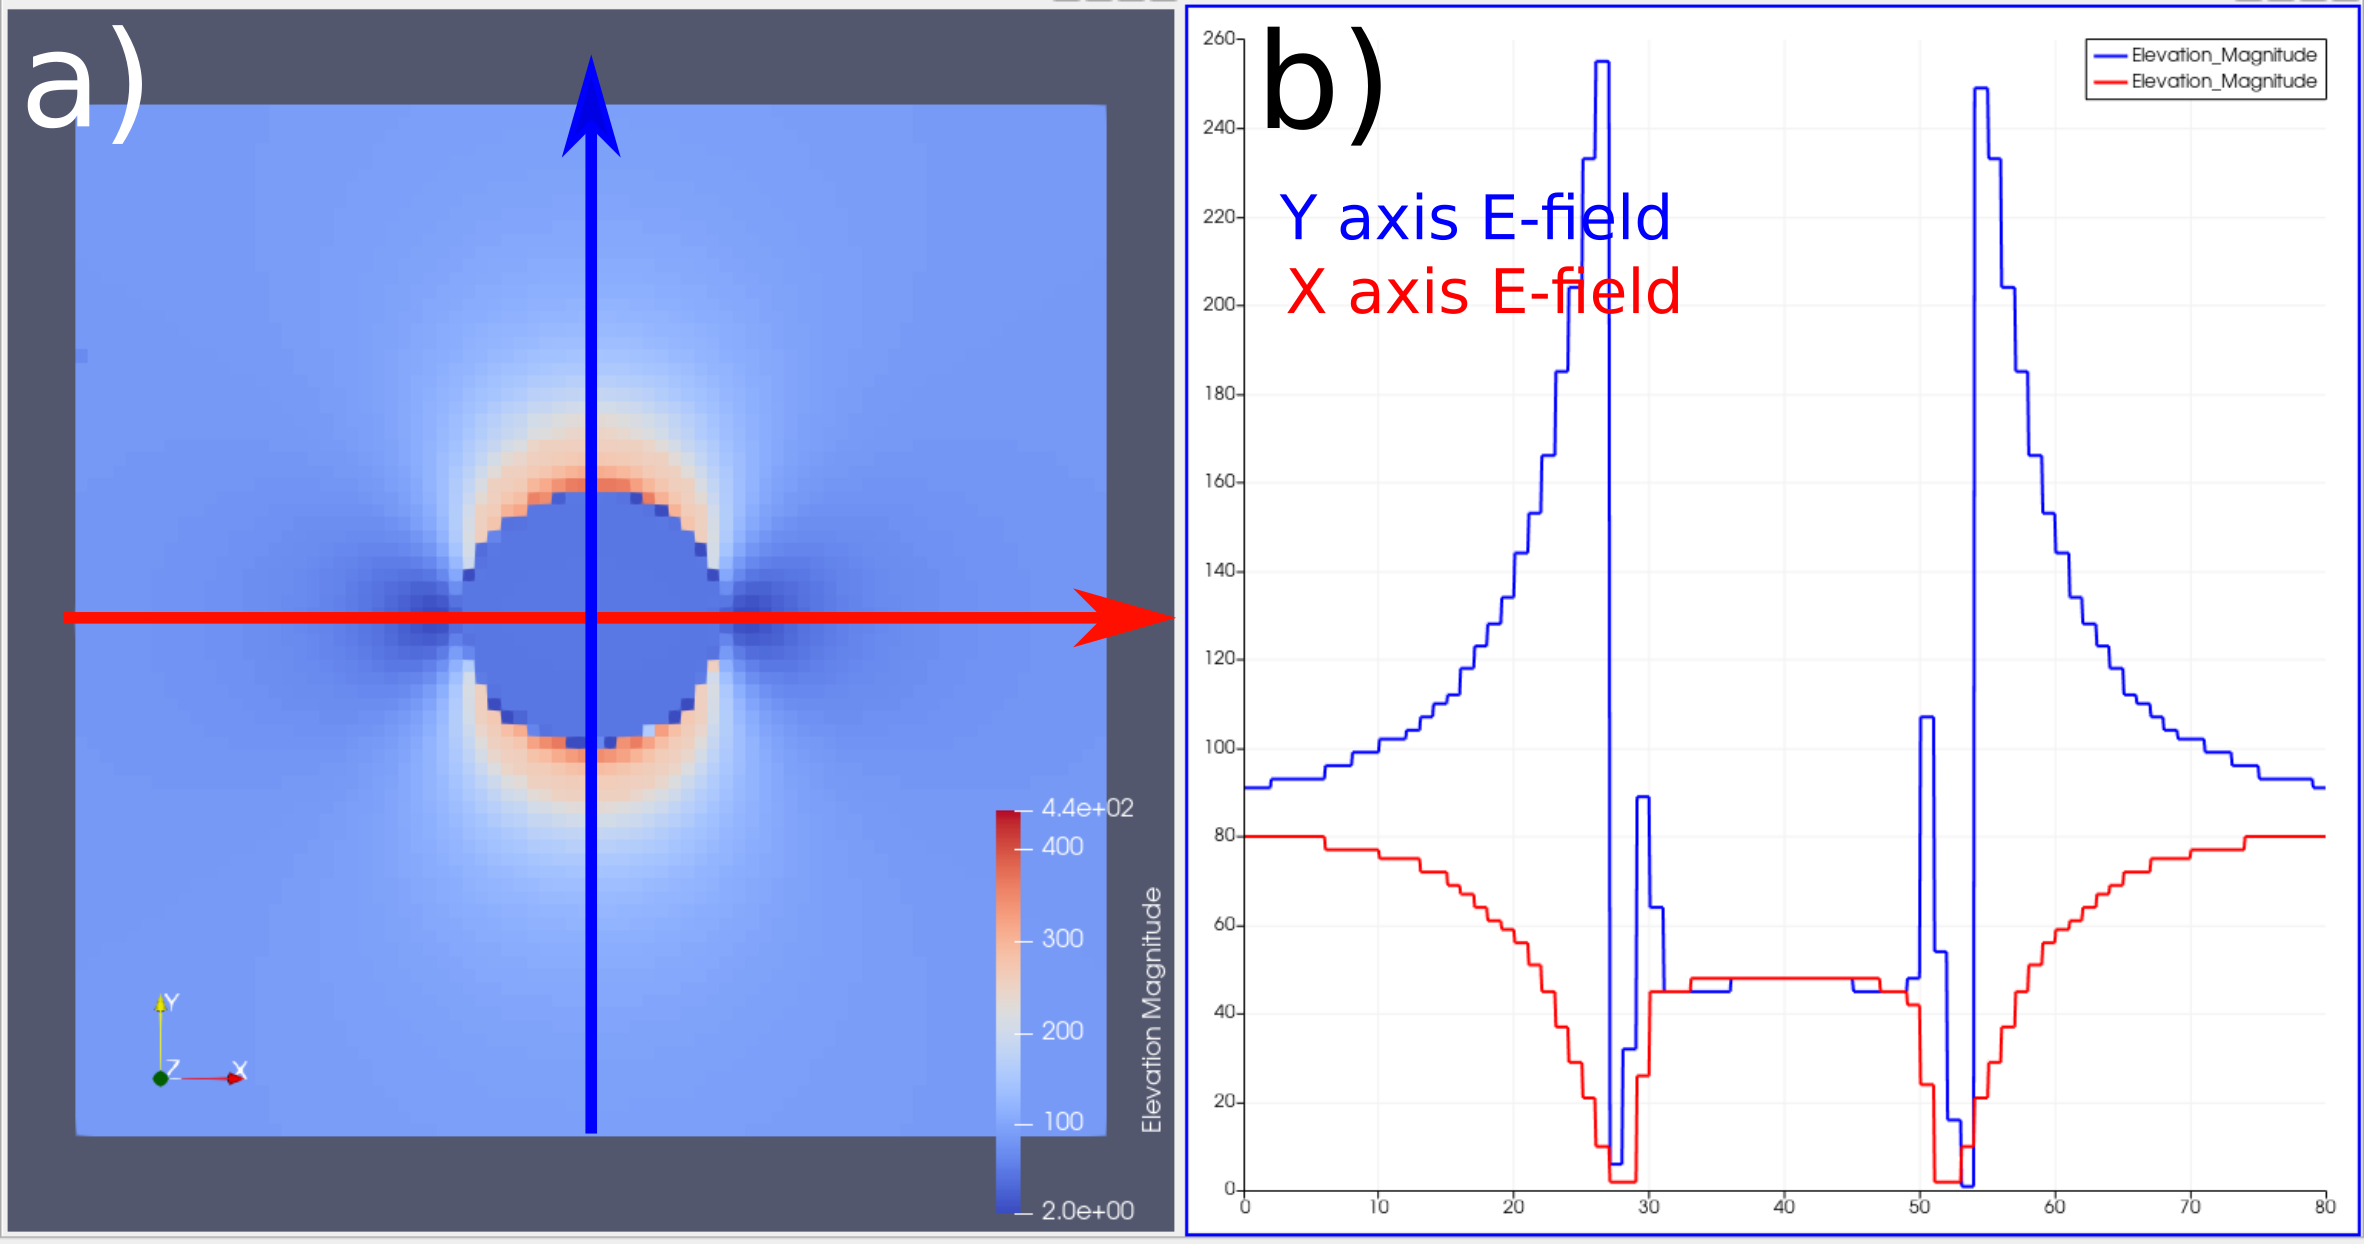
\includegraphics[width=0.7\textwidth]{mnpbem.png}
		\caption{(a) electric field magnitude around a 20 nm sphere calculated MNPBEM toolbox. (b) electric field variation along x and y axes. (test id3)} \label{mnpbem} 
	\end{figure}

    Figure \ref{testid3-1}  compares the \progname{} electric field magnitude calculated for the nanoshells of different mesh densities with MNPBEM results. According to this result \progname{} at the moment cannot properly calculate electric field magnitude in the space. It is expected that improving mesh density improves the response but this cannot be concluded from results in Figure \ref{testid3-1}.  
    
    \begin{figure} \centering 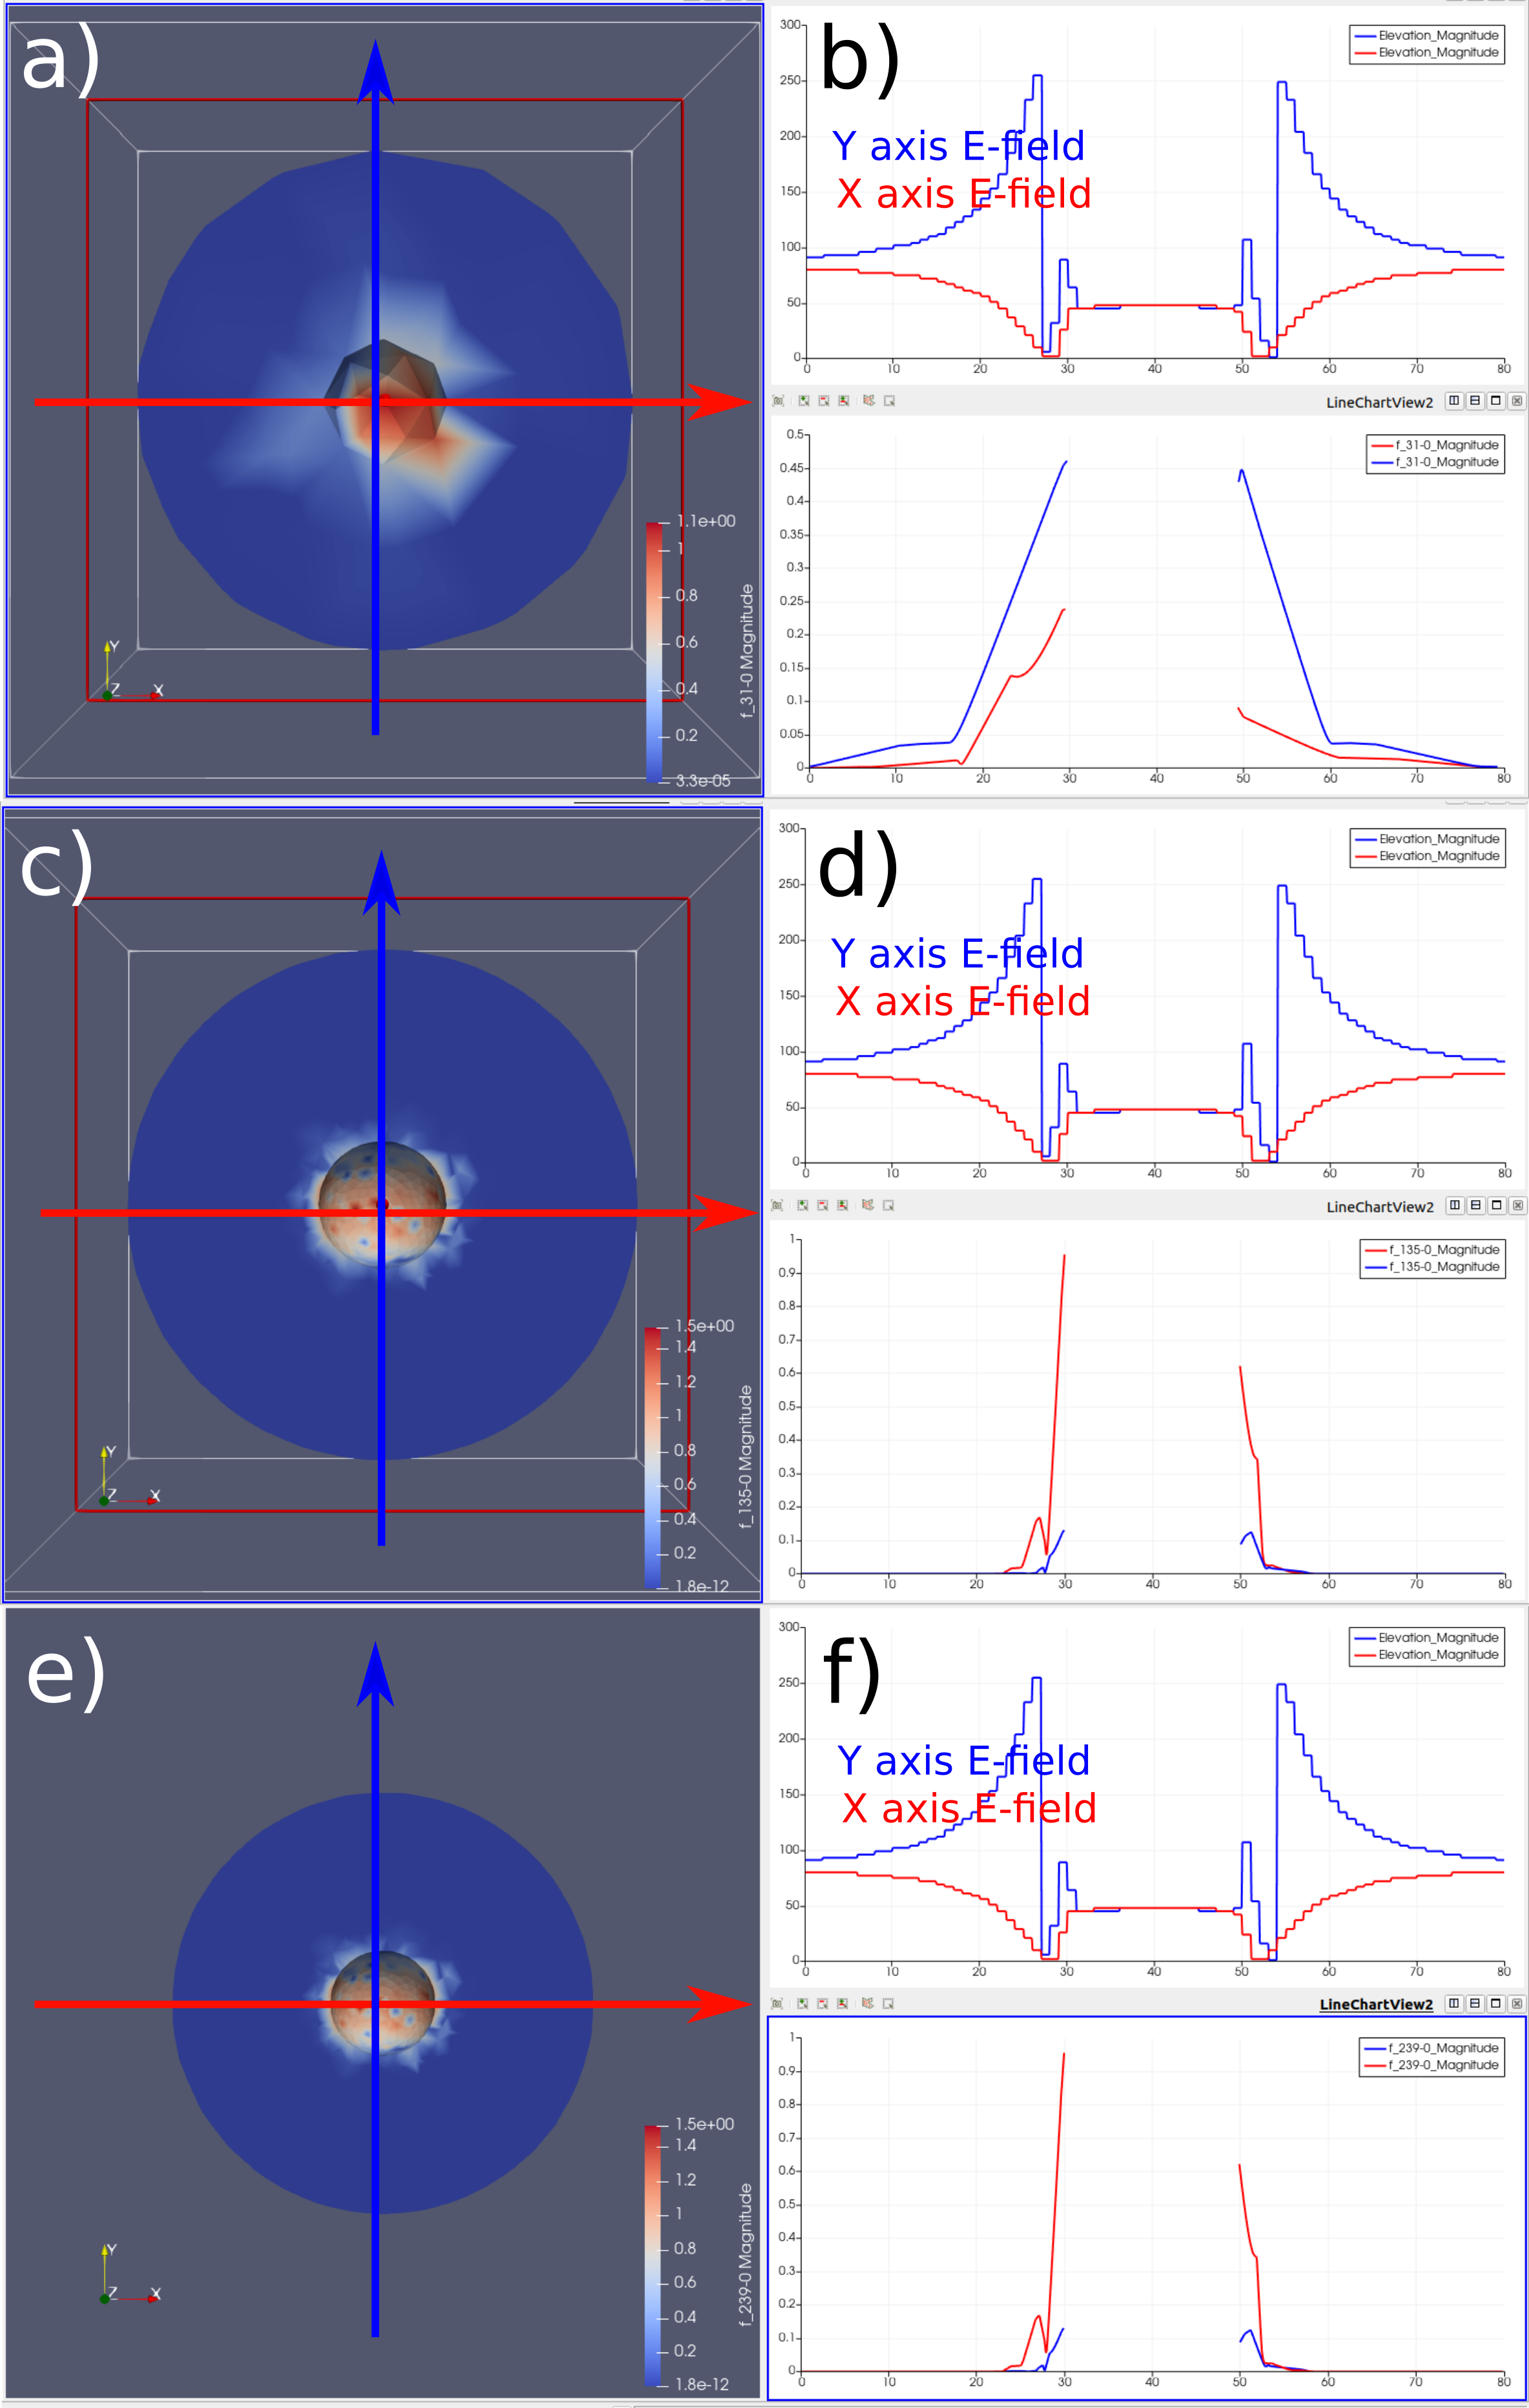
\includegraphics[width=0.7\textwidth]{testid3-shell.png}
    	\caption{(a), (c), and (e) show electric field magnitude around a 20 nm hollow spheres with respectively low, medium, and high mesh densities, calculated by \progname{}. (b), (d), and (f) plot electric field magnitude along x and y axis of the \progname{} calculations at the bottom and compares it with the obtained result from MNPBEM simulations on top (test id3)} \label{testid3-1} 
    \end{figure}

    In Figure \ref{testid3-2} similar data is depicted for a fully meshed nanoparticle. Although the response in low density mesh and high mesh density resembles the data from MNPBEM and it also improves when mesh density is higher, for the structure with medium meshed density response is not as expected and understanding the source of error requires further investigations. The other abnormality in the \progname{} response is the opposite polarity of the electric field. Considering the fact that light propagation direction is parallel to x-axis (red arrow), it is expected to see electric field enhancement in the orthogonal direction (blue axis). This error also needs to be subject further investigation. However, in general the response of \progname appears to be more promising when the whole geometry is meshed. 

    \begin{figure} \centering 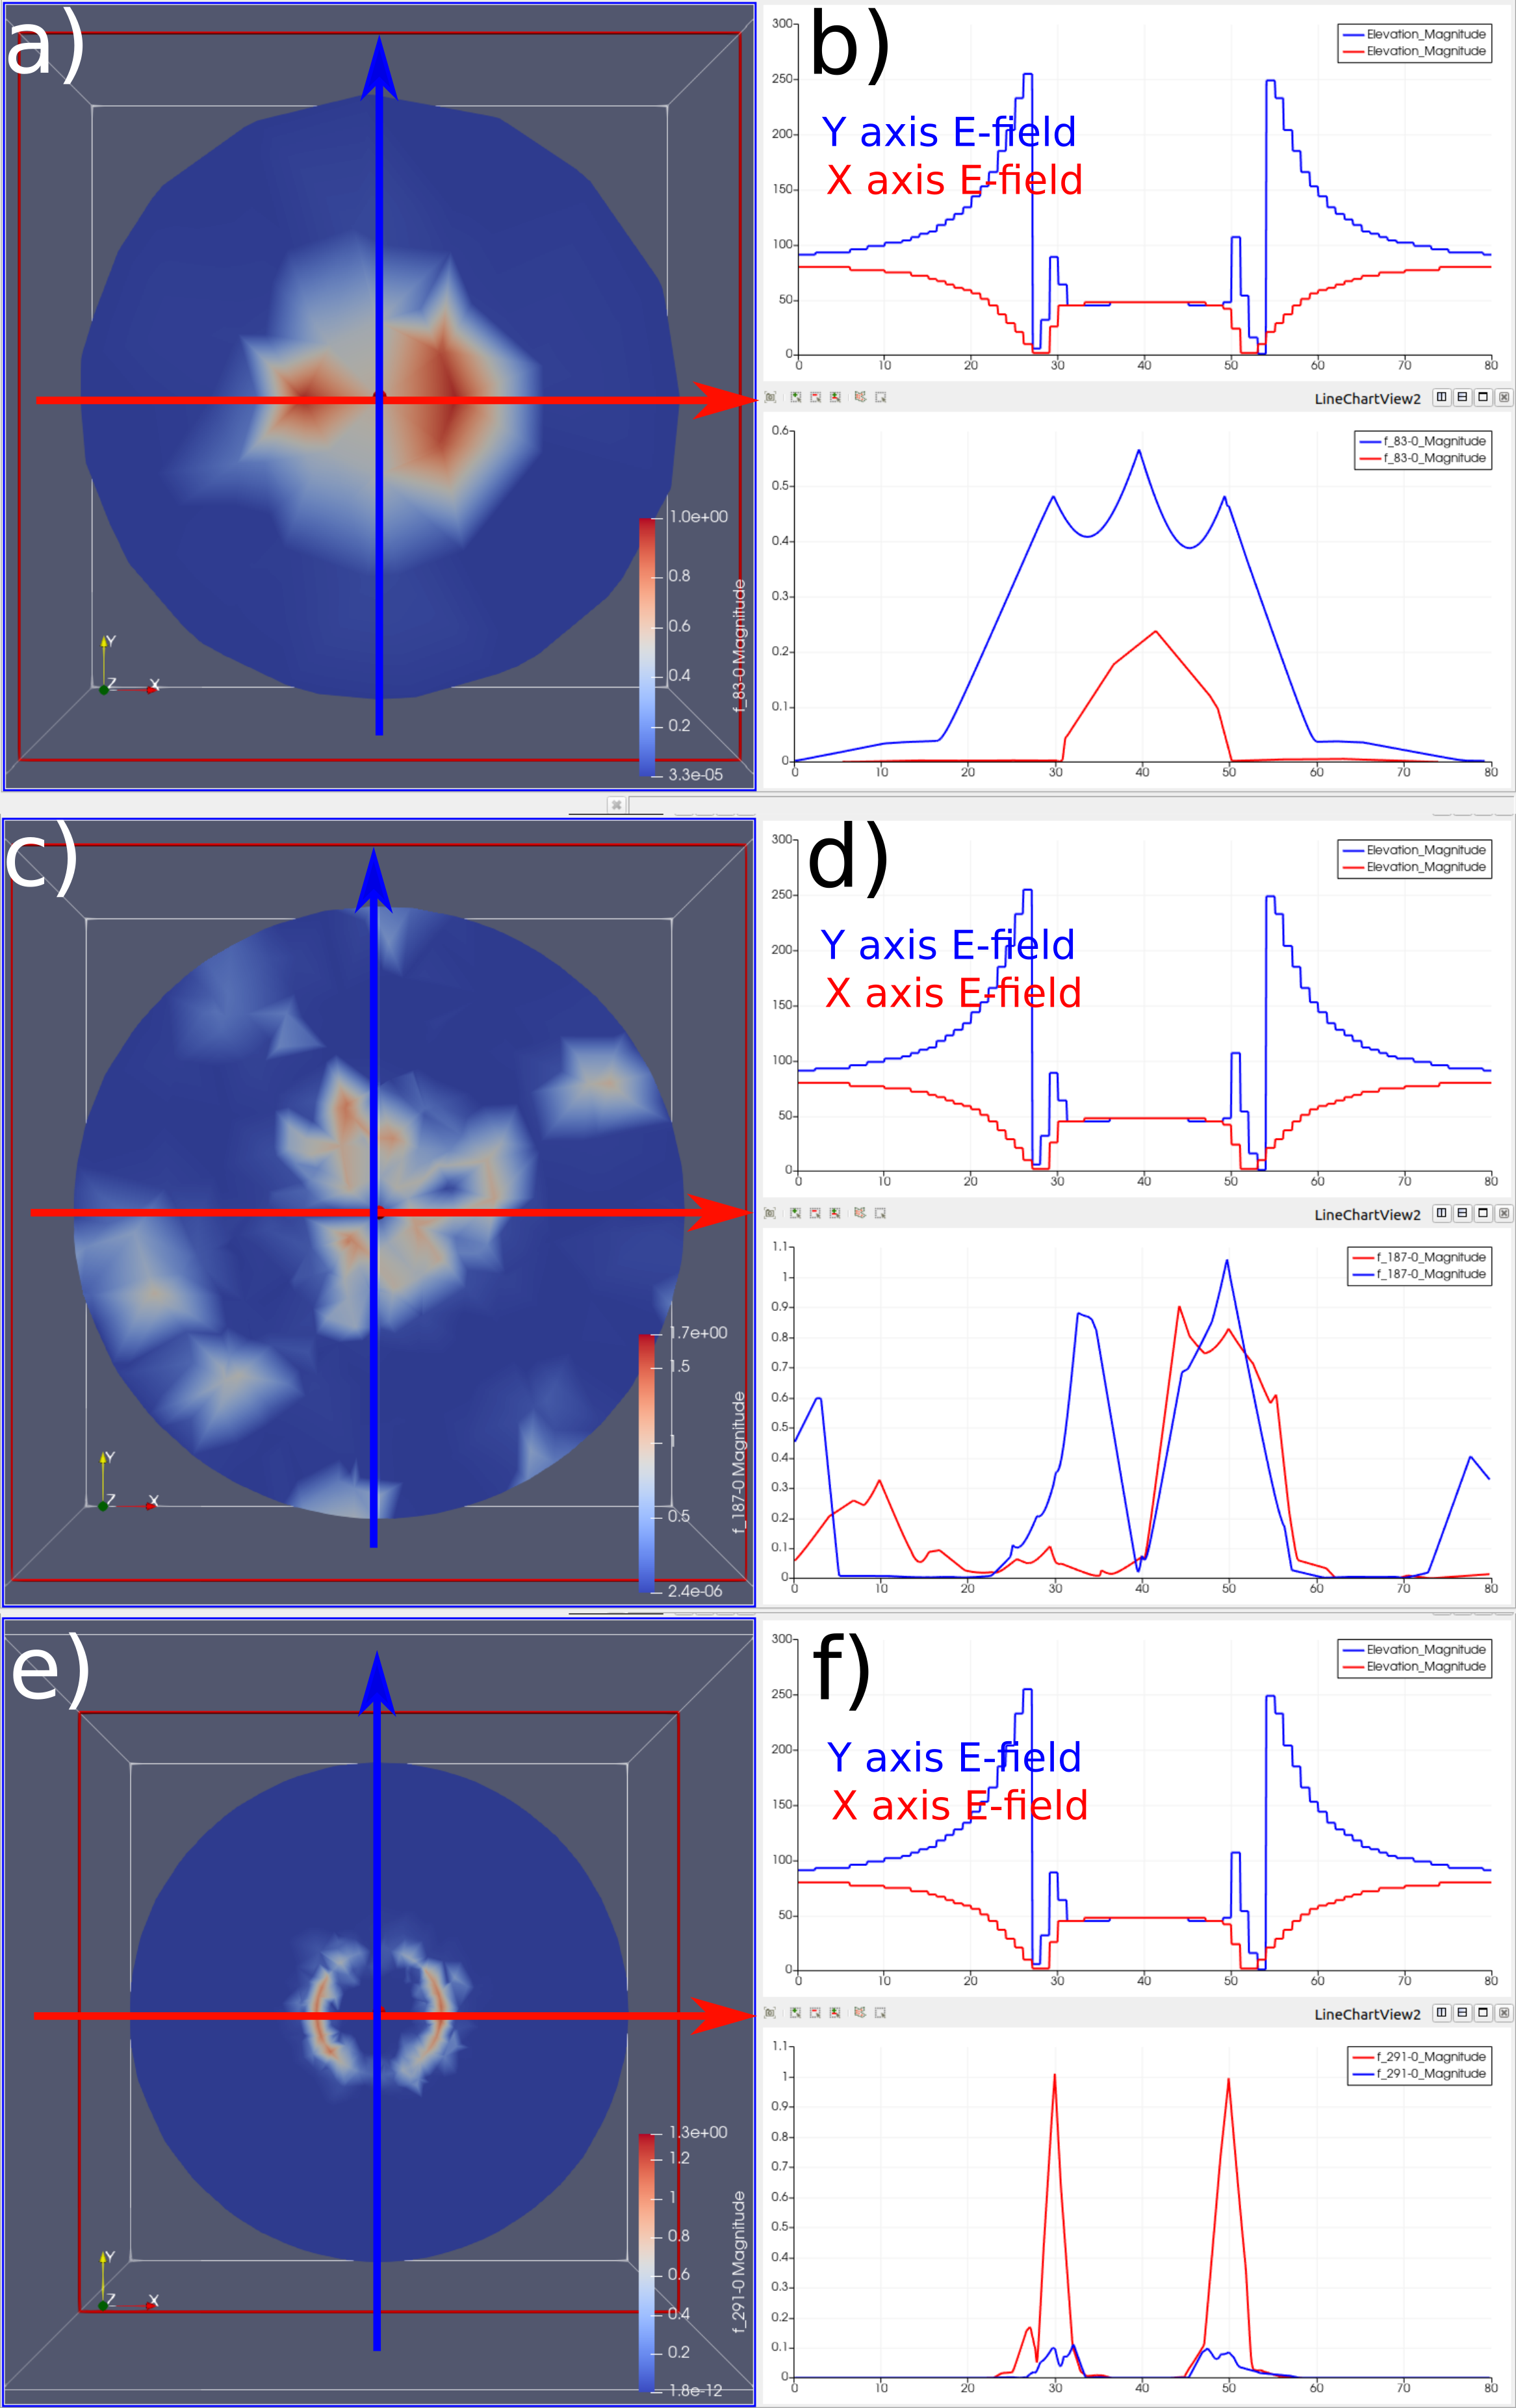
\includegraphics[width=0.7\textwidth]{testid3-fill.png}
	\caption{(a), (c), and (e) show electric field magnitude around a 20 nm thoroughly meshed spheres with respectively low, medium, and high mesh densities, calculated by \progname{}. (b), (d), and (f) plot electric field magnitude along x and y axis of the \progname{} calculations at the bottom and compares it with the obtained result from MNPBEM simulations on top (test id3)} \label{testid3-2} 
\end{figure}

Figure \ref{testid3-time} shows the execution time in the studied models in Test id3 and as is evident increasing the execution time non-linearly. Comparing Figure \ref{testid3-time} with Figure \ref{test1nodes}, where number of nodes were much higher, shows that the FEM solver, as expected, is extremely slower during solving equations than when it sets up the light source using interpolation. This data would have been useful if \progname{} result were more promising and could help user find an optimum between accuracy of result, execution time, and the mesh density. This stream will be definitely pursued in the future but at the moment the goal is to make \progname functional.

\begin{figure} \centering 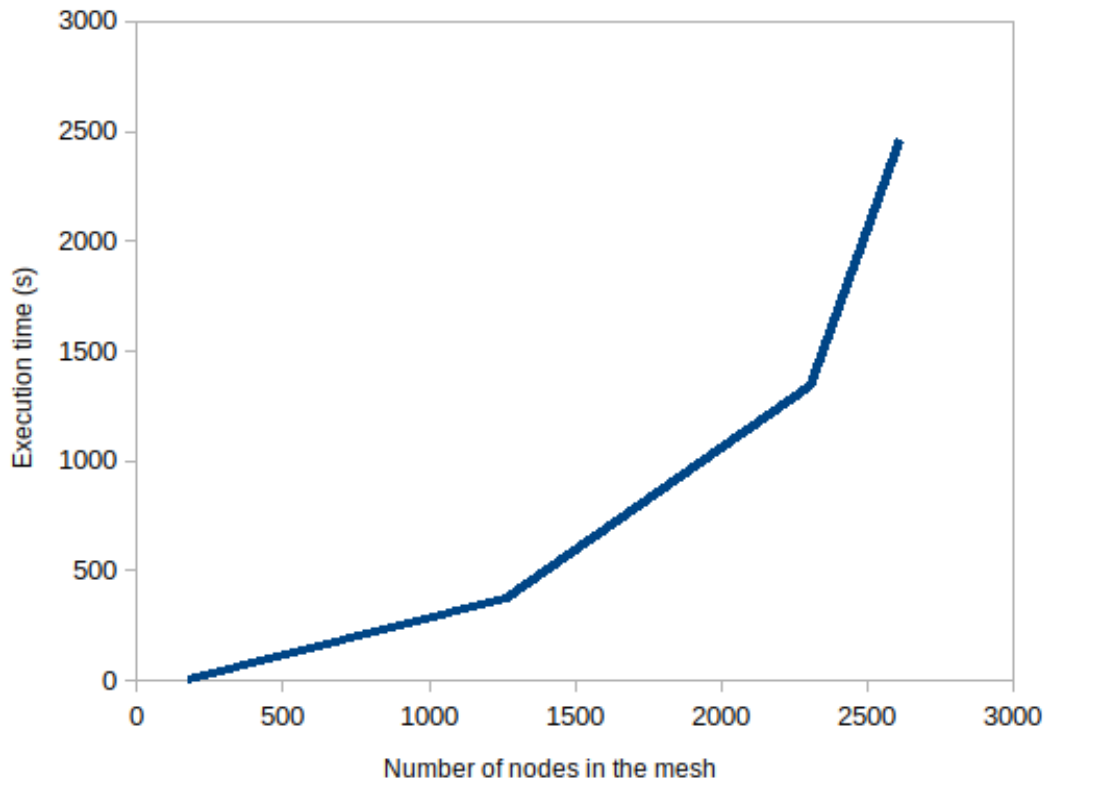
\includegraphics[width=1\textwidth]{testid3-time}
	\caption{\progname execution time for simulation of similar systems with different mesh densities (number of nodes in the mesh).} \label{testid3-time} 
\end{figure}



	\item{\textbf{Test id4:} plasmon enhanced electric field calculation\\}
	
	Implementation of this test is beyond scope of this document and it requires a wider time-frame. This test is postponed for the next year (2021).
	
\end{enumerate}
\subsection{Tests for Nonfunctional Requirements}
\label{nonfunc}

\subsubsection{Usability}
		
\paragraph{Test NR1: Capability of execution of the software}

\begin{enumerate}

\item{\textbf{Test id5:} Usability \\}

As the author has not yet received any response according to usability surveys reporting about this area is postponed to the future drafts of the present document. 

\end{enumerate}

\subsubsection{Maintainability}

\paragraph{Test NR2: Maintainability and expandability of the software}

\begin{enumerate}
	
	\item{\textbf{Test id6:} Maintainability\\}
	
	As author has not yet received surveys regarding the maintainability of \progname{}, reporting the results regarding this area of the software will be postponed to the future drafts of the current document. 
					
\end{enumerate}


\section{Unit Tests} \label{utest}

\subsection{Tests for Functional Requirements}

\subsubsection{Module 4: Constant parameters module (M4)}
\begin{enumerate}
	\item{\textbf{Test id7}  \\}
	
	By executing \href{https://github.com/shmouses/SPDFM/tree/master/src/test_const.py}{test\_const.py} using Pytest this module is tested and verified. 
\end{enumerate}
\subsubsection{Module 5: Input parameters modules (M5)}

\begin{enumerate}
	
	\item{\textbf{Test id8}  \\}
	
	By execution of  \href{https://github.com/shmouses/SPDFM/tree/master/src/test_inputparam.py}{test\_inputparam.py}, using Pytest in python, performance of this module tested and verified.
	
\end{enumerate}


\subsubsection{Module 6: Input Mesh modules (M6)}

\begin{enumerate}
	\item{\textbf{Test id9}\\}
	By executing \href{https://github.com/shmouses/SPDFM/tree/master/src/test_inputmesh.py}{test\_inputmesh.py} and visual inspection this module tested and verified. 
\end{enumerate}

\newpage

\bibliographystyle{plainnat}

\bibliography{../../refs/References}

\end{document}